\documentclass[tikz]{standalone}%

\usepackage[utf8]{inputenx}%  http://ctan.org/pkg/inputenx
% Euler for math | Palatino for rm | Helvetica for ss | Courier for tt
\renewcommand{\rmdefault}{ppl}% rm
\linespread{1.05}% Palatino needs more leading
\usepackage[scaled]{helvet}% ss //  http://ctan.org/pkg/helvet
\usepackage{courier}% tt // http://ctan.org/pkg/courier
\usepackage{eulervm}  %  http://ctan.org/pkg/eulervm
% a better implementation of the euler package (not in gwTeX)
\normalfont%
\usepackage[T1]{fontenc}%  http://ctan.org/pkg/fontenc
\usepackage{textcomp}%  http://ctan.org/pkg/textcomp

\usetikzlibrary{decorations.markings}
\usetikzlibrary{calc}

\begin{document}
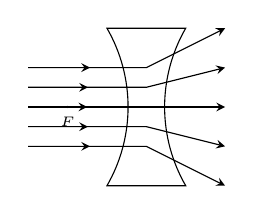
\begin{tikzpicture}
  \pgfmathsetmacro{\lH}{1}
  \pgfmathsetmacro{\lR}{2}
  \pgfmathsetmacro{\sA}{asin(\lH/\lR)}
  \pgfmathsetmacro{\base}{1}
  \pgfmathsetmacro{\xshi}{\base/2}
  
  \draw[yshift = -2cm, xshift = -\xshi cm] (0, \lH cm)
  arc[start angle = -\sA, delta angle = 2*\sA, radius = \lR cm] --
  +(\base cm, 0)
  arc[start angle = 180 - \sA, delta angle = 2*\sA, radius = \lR cm]
  -- cycle;

  \fill[fill = black] (-1cm, 0) coordinate (F) circle[radius = 0.015cm]
  node[below, font = \tiny] {$F$}; 

  \begin{scope}[decoration = {
      markings,
      mark = at position 0.3 with {\arrow{stealth}}
    }
    ]
    \foreach \y in {0.5, 0.25, 0, -0.25, -0.5}{
      \draw[postaction = decorate, -stealth] (-1.5cm, \y cm) -- (0, \y cm)
      coordinate (A) -- ($(F)!2!(A)$);
    }
  \end{scope}
\end{tikzpicture}
\end{document}
%%% Local Variables:
%%% mode: latex
%%% TeX-master: t
%%% End:
